\chapter{Methode}

\section{Algoritmen}

Eerder in deze scriptie (sectie \ref{bestaande-methoden}) hebben we een korte inleiding gegeven tot de voornaamste methoden waarmee datastreams gesynchroniseerd kunnen worden. Hoewel de meeste algoritmen niet voldeden aan onze vereiste waren er toch twee die ons wel bruikbaar leken voor snelle en nauwkeurige synchronisatie van realtime streams. In dit gedeelte zullen deze methoden in detail worden behandeld. Vervolgens onderzoeken we in welke mate het mogelijk is om deze algoritmes te combineren in één systeem.

\subsection{Accoustic fingerprinting}

Zoals in de introductie al is beschreven maakt het accoustic fingerprinting algoritme gebruik van fingerprints geëxtraheerd uit audiofragmenten. Het op zoek gaan naar gelijkenissen gebeurt door deze fingerprints met elkaar te vergelijken. Hoe dit precies in zijn werk gaat en hoe het mogelijk is om met deze techniek de latency tussen audiofragmenten te bepalen zal hieronder worden verklaart.

\subsubsection{Werking}
\begin{figure}[h]
	\captionsetup{width=\textwidth}
	\caption[Schema synchronisatie met fingerprinting]{Schematische voorstelling van synchronisatie met behulp van een accoustic fingerprinting systeem.}
	\advance\parskip0.5cm
	\begin{tikzpicture}[overlay]
\node at (-1,0) [minimum width=2cm] (A) {};

\node (rect) at (3,0) [draw,thin,minimum width=3cm,minimum height=1cm,align=center,font=\footnotesize] (B) {Feature \\[-0.7em] extractie};

\node (rect) at (8,0) [draw,thin,minimum width=3cm,minimum height=1cm,align=center,font=\footnotesize] (C) {Fingerprint \\[-0.7em] constructie};

\node (rect) at (13,-2) [draw,thin,minimum width=3cm,minimum height=1cm,align=center,font=\footnotesize] (G) {Andere \\[-0.7em] fingerprints};

\node (rect) at (13,0) [draw,thin,minimum width=3cm,minimum height=1cm,align=center,font=\footnotesize] (D) {Matchen en \\[-0.7em] bepalen latency};

\node at (17,0) [minimum width=2cm] (E) {};

\node at (0,-10) [minimum height=5cm] (F) {};

\draw [->] (A) -- (B) node [pos=0.4,above,align=center,font=\footnotesize] {Buffer};
\draw [->] (B) -- (C) node [pos=0.5,above,align=center,font=\footnotesize] {Features};
\draw [->] (C) -- (D) node [pos=0.5,above,align=center,font=\footnotesize] {Fingerprint};
\draw [->] (D) -- (E) node [pos=0.6,above,align=center,font=\footnotesize] {Latency};
\draw [->] (G) -- (D);

\end{tikzpicture}
	\advance\parskip1cm
\end{figure}
\vspace{2.5cm}

De cruciale stap bij de ontwikkeling van een accoustic fingerprinting systeem is het bepalen van de meest betrouwbare \textit{feature} om de fingerprints op te baseren. Mogelijke features zijn frequentie, toonhoogte, tempo, ritme, dynamiek, etc. Veel features zijn echter moeilijk (softwarematig) te bepalen wat hen niet bruikbaar maakt in een robuust fingerprinting systeem. Een feature die wel geschikt is voor het bepalen van fingerprints zijn de pieken in het frequentiespectrum.

\begin{figure}[!h]
	\caption[Voorbeeld van een spectrogram]{Spectrogram van Venetian Snares - Look}
	\centering
	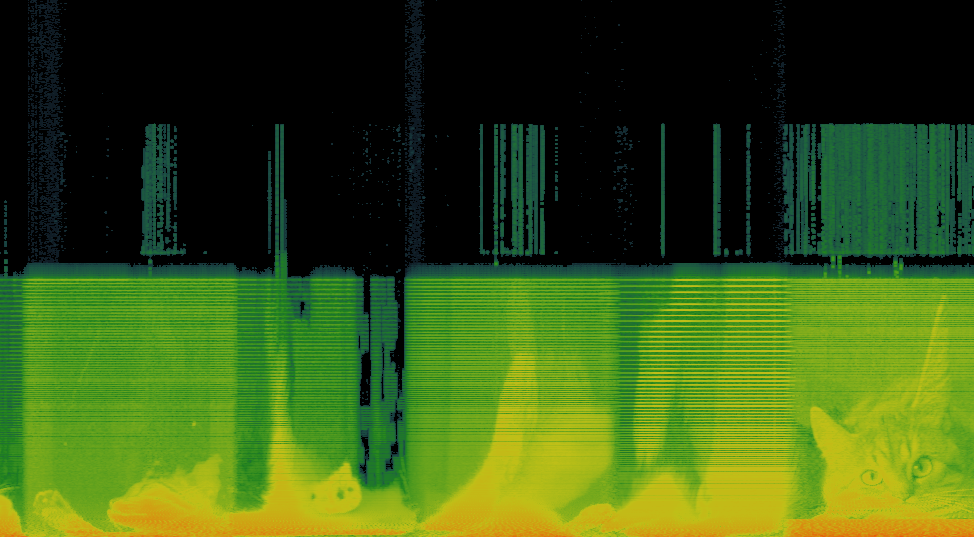
\includegraphics[width=0.5\textwidth]{spectrogram3.png}
\end{figure}
Een fingerprinter gebaseerd op de extractie van spectrale pieken gaat in verschillende stappen te werk: 
Eerst wordt er van elk audiofragment een spectrogram\footnote{Een spectrogram is een grafische voorstelling van de frequentie en intensiteit van geluid ten opzicht van de tijd \cite{spectrogram_dict}} gegenereerd. Dit kan snel gebeuren met het Fast Fourrier Transformation algoritme (FFT). In artikel \cite{oppenheim1970speech} wordt deze methode uitgebreid besproken. Vervolgens worden de fingerprints bepaald door telkens twee pieken in het spectrogram te verbinden. Een tijd-frequentie punt in het spectrogram is een kandidaat-piek als het punt een hogere energetische waarde heeft dan al zijn buren \cite{Wang2003a}. Welke pieken precies met elkaar worden verbonden hangt af van verschillende parameters.

Na het bepalen van de fingerprints worden ze opgeslagen in een datastructuur waarin er snel naar matches kan worden gezocht.
Van elke fingerprint worden volgende parameters bepaald:
\begin{itemize}[noitemsep]
	\item $ f1 $: de frequentie van de eerste spectrale piek van de fingerprint.
	\item $ t1 $: de tijd van de eerste spectrale piek van de fingerprint.
	\item $ \Delta f $: het verschil van de frequenties van beide spectrale pieken van de fingerprint.
	\item $ \Delta t $: het verschil in tijd van beide spectrale pieken van de fingerprint.
\end{itemize}

De fingerprints worden in volgende structuur bijgehouden: $ ( id; t1; hash(f1; \Delta f; \Delta t) ) $.

De hash wordt gebruikt om verschillende fingerprints te kunnen matchen. Deze bevat $ f1 $ en $ \Delta f $ omdat bij een match de beginfrequentie en het verschil in frequentie van beide fingerprints gelijk moet zijn. Enkel $ \Delta t $ wordt bijgehouden aangezien de begintijd van beide fingerprints waarschijnlijk niet zal overeenkomen. Het verschil in tijd tussen de fingerprints moet wel overeenkomen.

\begin{figure}[h]
	\captionsetup{width=0.7\textwidth}
	\caption[De anatomie van een fingerprint]{De anatomie van een fingerprint in het tijd-frequentie domein. Met toestemming overgenomen uit artikel \cite{six2015multimodal}.}
	\begin{center}
		\advance\parskip0.3cm
		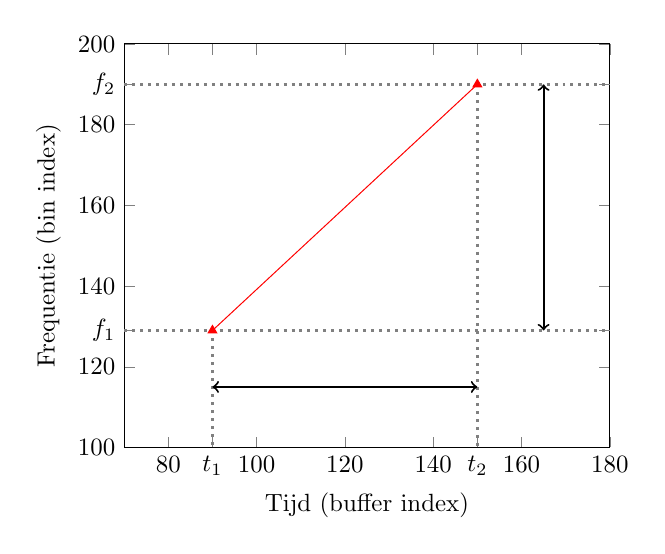
\begin{tikzpicture}[scale=0.9]
\begin{axis}[
	xlabel={Tijd (buffer index)},
	ylabel={Frequentie (bin index)},
	xmin=70,xmax=180,
	ymin=100,ymax=200,
	legend style={
  		cells={anchor=west},
  		legend pos=outer north east,
	},
	extra y ticks={129,190}, 
	extra y tick labels={$f_1$,$f_2$},
	extra x ticks={90,150}, 
	extra x tick labels={$t_1$,$t_2$},
]

  % plot the data from the file data.dat
  % smooth the curve and mark the data point with a dot
  \addplot[color=red,mark=triangle*] coordinates {
  	(90,129)
  	(150,190)
  };
  
  %f1
   \addplot[style= dotted,color=gray,very thick] coordinates{ (70,129)
   (180,129)};
   %f2
   \addplot[style= dotted,color=gray,very thick] coordinates{ (70,190)
   (180,190)};
   
    \node at (99,60) [] {\small$\Delta f$};
    \addplot[color=black,<->,thick] coordinates{ (165,129) (165,190)};
    
   \node at (50,18) [] {\small$\Delta t$};
   \addplot[style=dotted,color=gray,very thick] coordinates{ (90,129)
   (90,100)}; 
   \addplot[style=dotted,color=gray,very thick] coordinates{
   (150,190) (150,100)};
   \addplot[color=black,<->,thick] coordinates{ (90,115)
   (150,115)};
  
  \end{axis}
\end{tikzpicture}
	\end{center}
\end{figure}

Na het extraheren en opslaan van de fingerprints kunnen er matches gezocht worden door de hashwaarden van de fingerprints van beide audiofragmenten met elkaar te vergelijken. Van elke match wordt de offset berekend, wat het verschil is tussen $ t1 $ van beide fingerprints. Wanneer beide fragmenten overeenkomen zal dit resulteren in een groot aantal matches met dezelfde offset. 

Accoustic fingerprinting kunnen we toepassen op streams door ze te bufferen. Na het opbouwen van de buffers dient het algoritme hierop te worden uitgevoerd. De maximale offset die gevonden werd bij het matchen komt overeen met de latency tussen beide streams.

Een uitgebreidere beschrijving is te vinden in artikel \cite{Wang2003a}. Deze methode is echter beperkt tot het vergelijken van audiofragmenten die in tijd noch toonhoogte gewijzigd zijn. Aan het IPEM is een aangepaste methode ontwikkeld die dit wel toelaat \cite{six2014panako}.

\subsubsection{Toepassing in realtime}

Door het bufferen van de streams kan accoustic fingerprinting gebruikt worden in een realtime toepassing. Afhankelijk van de gebruikte parameters en de kwaliteit van de audio is een buffergrootte van enkele seconden voldoende om de latency tussen de streams te bepalen. Verder in dit hoofdstuk zal het bufferen worden besproken.

De nauwkeurigheid van dit algoritme hangt af van de grootte van de \textit{FFT bins}. De waarde hiervan is afhankelijk van de parameters van het FFT algoritme. Een nauwkeurigheid van 16 ms of 32 ms is standaard.

\subsection{Kruiscovariantie}

Deze methode bepaalt de gelijkenis tussen twee audiofragmenten en resulteert in een bepaalde. De latency tussen twee audiofragmenten kan bepaald worden door deze berekening uit te voeren voor elke mogelijke verschuiving. De verschuiving waarbij de kruiscovariantie het hoogst is bepaalt de latency.

\subsubsection{Werking}

Stel twee audioblokken $ a $ en $ b $ bestaande uit $ s $ samples en verschuiving $ i $. Voor elke $ i $ gaande van 0 tot $ s $ wordt de kruiscovariantie berekent met volgende formule:

\begin{equation}
\sum_{j=0}^{s} a_{j} \cdot b_{(i+j)\ mod\ s}
\end{equation}

De waarde van $ i $ waarbij de kruiscovariantie het hoogst is stelt de latency voor tussen beide audioblokken in aantal samples. De latency in seconden bepaalt men door dit resultaat te delen door de samplefrequentie.

De methode kan de latency tot op één sample nauwkeurig bepalen. De maximaal bereikbare nauwkeurigheid hangt dus af van de samplefrequentie van de audioblokken. Bij een samplefrequentie van $8000 Hz$ is dit $ 1/8000 Hz = 0.125 ms $. Dit is ruim voldoende voor onze toepassing.

Een nadeel aan deze methode is de performantie. Het berekenen van de beste kruiscovariantie van twee audioblokken bestaande uit s samples kan gebeuren in  $O(s^{2})$. Het is dus belangrijk om bij deze berekening de grootte van de audioblokken te beperken.

In artikel \citealp{six2015multimodal} wordt deze techniek meer in detail besproken.

\subsubsection{Toepassing in realtime}

Het bufferen van de audiostreams maakt ook dit algoritme in realtime toepasbaar. In tegenstelling tot accoustic fingerprinting is het niet de bedoeling dat de berekeningen op de volledige buffer wordt uitgevoerd. Door de kwadratische tijdscomplexiteit zou dit onnoemelijk veel rekenkracht vragen.\footnote{Voor het berekenen van de kruiscovariantie tussen twee buffers met $10s$ audio en een samplefrequentie van $8000hz$ zijn er asymptotisch 6400000000 berekeningen vereist.} Hoe de berekening dan wel moet worden uitgevoerd wordt verderop uitgelegd.

\subsection{Toepasbaarheid}

Het accoustic fingerprinting algoritme is zeer snel en robuust en kan gebruikt worden om gebufferde audiostreams te synchroniseren tot enkele tientallen milliseconden nauwkeurig (afhankelijk van de parameters van het FFT algoritme).

Het kruiscovariantie algoritme kan eveneens gebruikt worden om (gebufferde) audiostreams te synchroniseren. De grootste troef van dit algoritme is haar nauwkeurigheid: in de beste omstandigheden kan het algoritme resultaten bekomen tot op één sample nauwkeurig. Het bereiken van een dergelijke nauwkeurigheid is onmogelijk met eender welk ander besproken algoritme. De keerzijde is de performantie van het algoritme. Bij het synchroniseren van grote audioblokken kan dit problematisch zijn.

De kenmerken van deze algoritmen zijn heel erg complementair. De gemakkelijkste manier om een robuust, snel én nauwkeurig systeem op te bouwen is door het beste van de twee werelden te combineren. Het accoustic fingerprinting algoritme kan zorgen voor de synchronisatie tot op enkele tientallen milliseconden nauwkeurig. Dit resultaat laat toe dat we het kruiscovariantie algoritme kunnen uitvoeren op zeer korte stukjes audio (een honderdtal milliseconden volstaat).

\section{Bufferen van streams}

\begin{figure}[h!]
	\captionsetup{width=0.7\textwidth}
	\caption[Schematische weergave van de buffer]{Schematische weergave van een verschuivende buffer over een audiostream.}
	\begin{center}
		\advance\parskip0.3cm
		\begin{tikzpicture}[scale=0.9]
\begin{axis}[
xlabel={Tijd (seconden)},
xmin=170,xmax=200,
ymin=0,ymax=1,
legend style={
	cells={anchor=west},
	legend pos=outer north east,
},
yticklabels={,,},
xticklabel style={grid=major},
extra x ticks={176,177,186,187},
extra x tick labels={,,,},
extra tick style={grid=major, grid style={dotted}},
hide y axis
]
\addplot[thick,black] graphics[xmin=140,ymin=0,xmax=200,ymax=1] {wave.png};

after end axis/.code={
	\draw[black,<->] (axis cs:175,0.1) -- (axis cs:185,0.1)	node [pos=0.5,above,font=\scriptsize] {buffer $i-1$};
	
	\draw[black,<->] (axis cs:176,0.2) -- (axis cs:186,0.2)	node [pos=0.5,above,font=\scriptsize] {buffer $i$};
	
	\draw[black,<->] (axis cs:177,0.3) -- (axis cs:187,0.3)	node [pos=0.5,above,font=\scriptsize] {buffer $i+1$};
}]

%\node at (50,18) [] {\small$\Delta t$};
%\addplot[style=dotted,color=gray,very thick] coordinates{ (90,129)
%	(90,100)}; 
%\addplot[style=dotted,color=gray,very thick] coordinates{
%	(150,190) (150,100)};
%\addplot[color=black,<->,thick] coordinates{ (90,115)
%	(150,115)};

\end{axis}

\end{tikzpicture}
	\end{center}
\end{figure}

Zowel in de introductie als bij de gedetailleerde bespreking van de algoritmes is er vaak aangehaald dat de streams gebufferd zullen worden. Hoe dit precies in zijn werk zal gaan is echter nog niet besproken. In dit deel wordt dit concept meer gedetaileerd uitgelegd.

Bij het bufferen maken we gebruik van een \textit{sliding window}. Deze techniek zorgt ervoor dat de algoritmes voldoende data hebben om berekeningen op uit te voeren terwijl wijzigingen aan de latency (door drift of gedropte samples) toch voldoende snel gedetecteerd worden.

De grootte van de buffer heeft invloed op de kwaliteit van de geretourneerde resultaten. Het is logisch dat de algoritmes de latency beter kunnen bepalen door 10s in plaats van 1s audio te analyseren. Een nadeel is echter dat het langer duurt vooraleer de latency of een wijziging ervan gedetecteerd kan worden. Indien er bijvoorbeeld buffers gebruikt worden die 10s audio kunnen bevatten, dan zal een wijziging aan de latency gemiddeld na iets meer dan 5 seconden gedetecteerd worden. Dit is te verklaren aangezien de buffer vanaf dat moment procentueel meer audio bevat met de gewijzigde latency dan audio met de oude latency.

In de evaluatiecriteria is er bepaald dat een wijziging aan de latency (door drift of gedropte samples) binnen één seconde gedetecteerd moet worden. Een verschuivende buffer kan hier voor zorgen: in plaats van een vast aantal seconden audio te bufferen en vervolgens de volledige grootte van de buffer op te schuiven wordt de buffer over een veel kleinere afstand verschoven. Hierdoor kunnen latencywijzigingen, ondanks de vertraging waarmee we de resultaten verkrijgen, toch nauwkeuriger en sneller bepaalt worden.
